\subsection{Calibration of the cars}
After building a second Raspberry Pi vehicle, we did some testing to figure out how the vehicles behaved together with the server when approaching an intersection. In this test, the vehicles were given a specific velocity and distance by the server. When the vehicles arrived at their destination, the server would tell them to stop and terminate their connection.

The vehicles were able to send information and respond correctly to the server's commands. We also observed that the vehicles drove a different length for each velocity given even though the length given by the server was the same. We assumed that the power given to the vehicle's motors equated to the velocity of the vehicle, which resulted in the unexpected behavior previously mentioned. The demonstration depended on the car's ability to input the correct amount of power to drive at specific speeds instructed by the server. Thus, the group started to measure the distance and time the cars would drive, given intervals of power to determine the relationship between power and velocity.

The measurement setup is as follows: The server instructs the cars to drive with a given power, which is what the server believed to be the velocity. After a time, the server will stop the car. The group then measured the distance the car had traveled. Given the measured distance and the time given by the server, the real velocity was obtained by dividing distance by time. \hyperref[tab:calibration]{Table \ref{tab:calibration}} shows all the recorded measurements with this set up.

\begin{table}[h!]
	\begin{center}
		\begin{tabular}{rrrr}
			\hline
			Power & Length (cm) & Time (s) & Velocity (cm/s) \\
			\hline
			40 & 467 & 8.98 & 52.00 \\
			50 & 425 & 7.28 & 58.38 \\
			60 & 400 & 6.06 & 66.01 \\
			70 & 357 & 5.18 & 68.92 \\
			80 & 325 & 4.49 & 72.32 \\
			90 & 314 & 4.03 & 77.92 \\
			100 & 286 & 3.62 & 79.01 \\
			\hline
		\end{tabular}
		\caption{Measurements taken to determine the relationship between power and velocity. Units were provided to the different parameters, while the power unit was unknown.}
		\label{tab:calibration}
	\end{center}
\end{table}

We then made a graph in Excel by plotting our data with velocity on the $y$-axis and power on the $x$-axis as shown in \figref{fig:graphvelpow}.

\begin{figure}[h!]
		\centering
	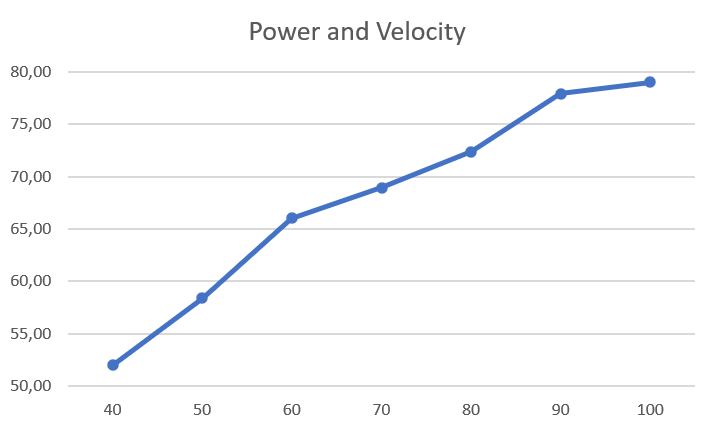
\includegraphics[width=1\linewidth]{figures/velocity_and_power}
	\caption[Graph of velocity as function of power]{Graph of velocity as a function of power}
	\label{fig:graphvelpow}
\end{figure}

From \figref{fig:graphvelpow}, it appears that the power and velocity were linearly correlated. Hence, using linear regression, we obtained an approximate relationship between power and velocity. \figref{fig:functionofpower} shows the result of the linear regression performed by Excel using the same dataset in \hyperref[tab:calibration]{Table \ref{tab:calibration}}.

\clearpage
\begin{figure}[h!]
	\centering
	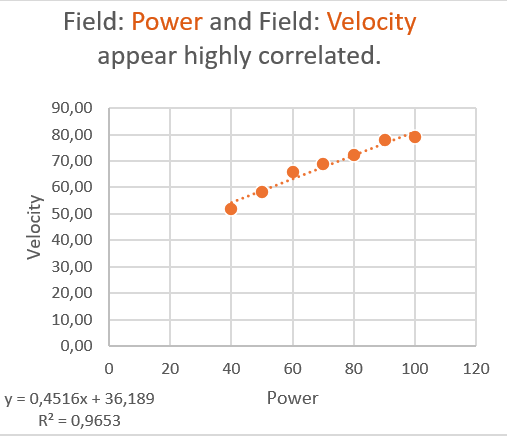
\includegraphics[width=1\linewidth]{figures/function_of_power}
	\caption{Graph of velocity as a function of power with linear regression in Excel. The x-axis shows the Power and the y-axis shows the velocity}
	\label{fig:functionofpower}
\end{figure}

From \figref{fig:functionofpower}, the relationship between velocity and power is as follows: 

\begin{equation}
	v(P) = 0.4516\cdot P + 36.189\label{eq:vprelationship}
\end{equation}

where $P$ is power and $v$ is velocity, with a goodness-of-fit measure of $R^2=0.9653$. We inserted the relationship into the vehicle and performed a new test to confirm the relationship. We observed that the vehicles drove more or less the correct distance for the desired velocity. Although the distance has some variance in the new tests, we concluded it was accurate enough for our demonstration. If, however, a more accurate formula is desired, then the test can be performed with smaller power intervals.

